\documentclass[11pt,a4paper]{article}
\usepackage[margin=2cm]{geometry}

%% adding graphics
\usepackage{graphicx}
%% nicer tables
\usepackage{booktabs}
%% rotate pages for landscape
\usepackage{pdflscape}
%% nice grid layouts for latex figures
\usepackage{subcaption}

\begin{document}

\title{Automatic Flow-based Classification of B-Cell Lymphoma}


\section{Introduction}

Flowcytometry aids in the detection and classification of lymphatic disorders, but current multi-channel flow data is hampered by the limitations of human interpretability.
Statistical preprocessing promises to enable the description of higher-dimensional relationships in measured events.
Extending previous work on preprocessing and classification of flowcytometry data, we created a proof-of-concept approach for unattended debris-removal and classification on a large dataset of B-Cell-Lymphoma.

\section{Aims}

Design and implementation of an automated analysis process for determination of B-Cell-Lymphoma diagnoses from flowcytometry data of peripheral blood and bone-marrow samples.


\section{Methods}

For the initial analysis flow cytometry data was obtained from routine flow panels for B-Cell-Lymphoma from the years 2016--2018. A total of xxx patients have been obtained. The given cohort contained 9 different B-Cell lymphoma subtypes, as well as non-pathological normal cases.

%% describe preprocessing, choronological in processing steps is easier to grasp

In order to focus the map on a cell population in question individual samples were preprocessed by automatically selecting a CD45 positive and side-scatter negative population using a density based clustering of individually generated SOMs.

A self-organizing map is trained on a sample of cases from all cohorts, creating a reference map of the data, we refer to as \emph{consensus-SOM}.
Invididual samples are afterwards sampled into the trained SOM and the distribution utilized for the classification into diagnoses in a sequential neural network.

%% describe classification process further


%% som based algorithm
%% consensus SOM
%% debris gating based on dbscan


\section{Results}

Initial 9-class classifications obtained accuracies of XX\% across 5 generated maps, with classification calculated in 10-fold cross-validation. Cohorts were at maximum limited to XX samples, while smaller cohorts were left at their respective sizes.
Hierarchical clustering showed similarities between CLL/PL and mantle cell lymphoma, as well as between lymphoplasmocytic lymphoma and marginal cell lymphoma.


\begin{figure}
   \centering
   \raisebox{-0.5\height}{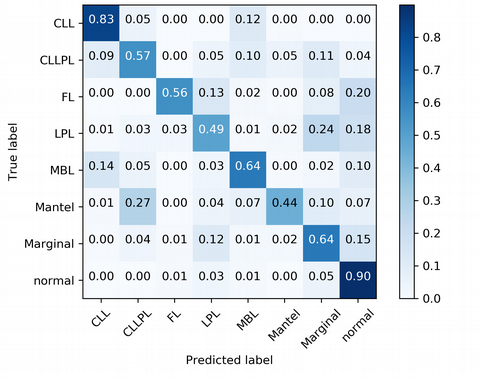
\includegraphics[width=0.5\textwidth]{dendro_confusion}}
   \raisebox{-0.5\height}{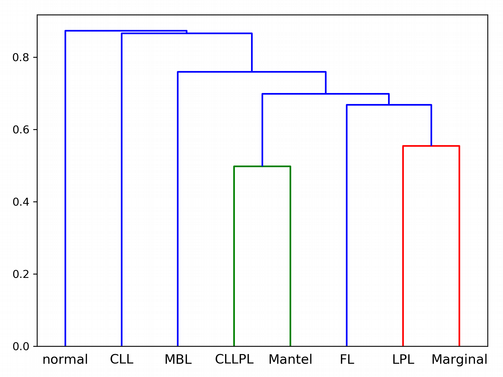
\includegraphics[width=0.4\textwidth]{dendro}}
   \caption{Hierarchical clustering on confusion matrix values. Groupings are created per column, with similar columns grouped closer.}
\end{figure}


%% tsne results and som for normal vs cll
%% pregating w/ dbscan
%% neural net classification normal cll
%% results for xxx different lymphoma entities
%% clustering joint entities, similarity in classification

\begin{figure}
   \caption{Classification results.}
\end{figure}

\begin{figure}
   \centering
   \raisebox{-0.5\height}{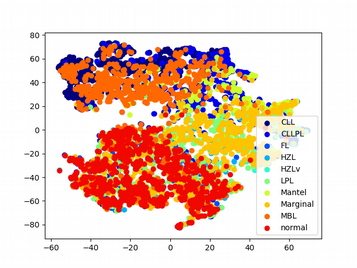
\includegraphics[width=0.45\textwidth]{tsne_t1}}
   \raisebox{-0.5\height}{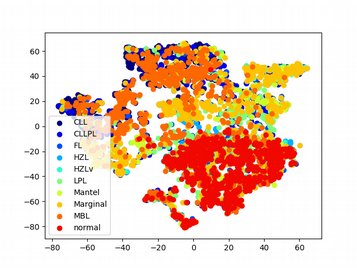
\includegraphics[width=0.45\textwidth]{tsne_t2}}
   \caption{tSNE visualization of upsampling histogram data from separated maps for tube 1 and tube 2.}
\end{figure}

\begin{figure}
   \caption{Pregating visualization}
\end{figure}

\section{Conclusions}

Our classification prototype shows the viability for automated classification on large routine diagnostics dataset.
Further improvements can be made to increase the flexibility of the approach to encompass incomplete and changing panels, as well as testing of a more diverse patient set, including cases with diagnoses outside the diagnostic target of given panel.

%% viability of automated conclusions

%% required further development

%% sources for error

%% combination approaches

%% challenges regarding changing data qualities etc

\end{document}
